\part{Medical Images Storage}

\chapter{Basic concepts}

\section{Storage media charactaristics}
\begin{enumerate}
\item \textbf{Capacity}: This is the total amount of data that a
  storage medium can hold. It's typically measured in \popup{B}{byte}s
  (8 \popup{bits, where a bit represents a logical state with one of
    two possible values.}), \popup{KB}{kilobyte}s
  ($1\text{KB} = 2^{10}\text{B}$), \popup{MB}{megabytes}s
  ($1\text{MB} = 2^{10}\text{KB}$), \popup{GB}{gigabyte}s
  ($1\text{GB} = 2^{10}\text{MB}$), \popup{TB}{terabyte}s
  ($1\text{TB} = 2^{10}\text{GB}$), and \popup{PB}{petabyte}s
  ($1\text{PB} = 2^{10}\text{GB}$).
\item \textbf{Volatility}: If the media need to connected to a current supply (for example, the \gls{RAM} memory of a computer), the media is said \emph{volatile}.
\item \textbf{\gls{WORM}}: A \gls{CDROM}, for example.
\end{enumerate}
\begin{itemize}
\item There are many storage media capable of storing digital images (some allow
\begin{enumerate}
\item 
\item Common massive storage systems (not only used for medical images) are:
\begin{enumerate}
\item \textbf{Cloud Storage} (Google Drive, Microsoft One Drive,
etc.): data is stored in remote servers accessed over the Internet.
\item \textbf{NAS (Network-Attached Storage)}: data is stored in a
\popup{specialized computer}{The computer rarely has a keyboard or
monitor, and has many hard drive bays.} (connected to the
\popup{LAN}{Local Area Network.}) that usually mounts several disks
with some type of \popup{RAID}{Redundant Array of Independent Disks.}
configuration.
\end{enumerate}
\end{itemize}
\vspace{-4ex}
\begin{figure}[!b]
  \centering
  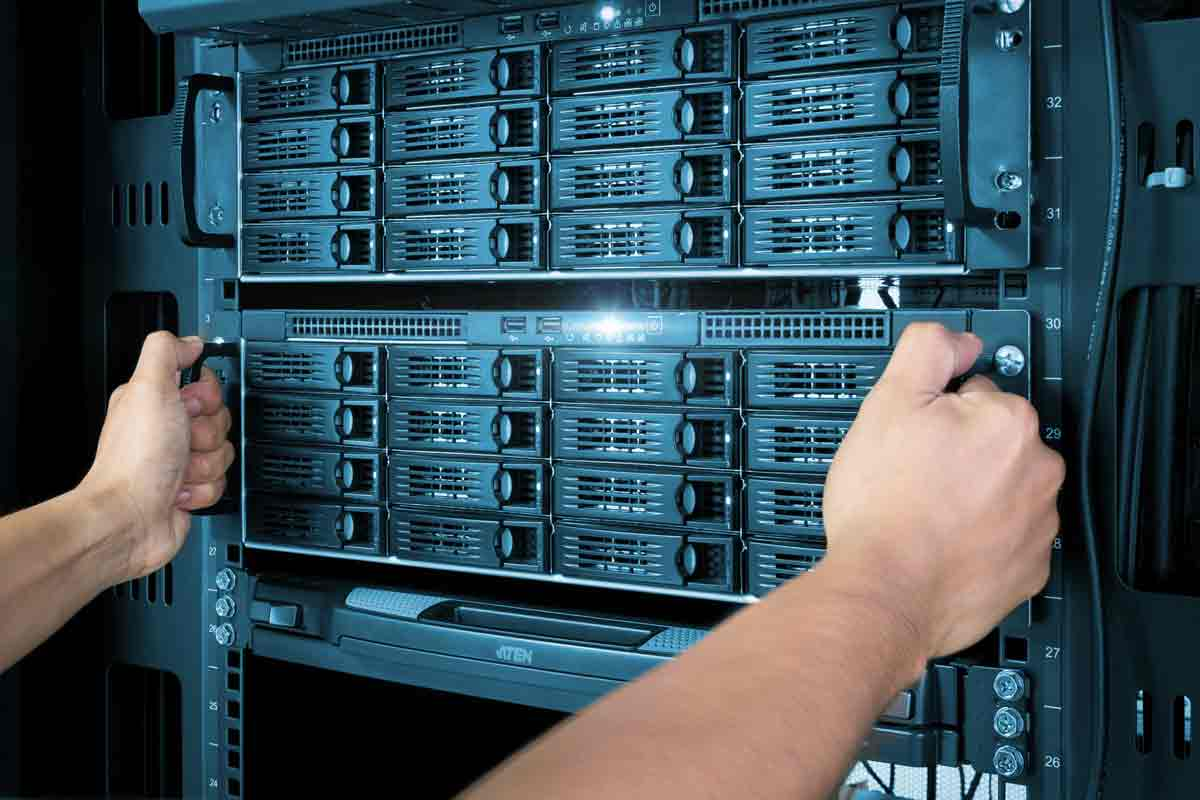
\includegraphics[height=3.5cm]{servidor-nas}
  \caption{A NAS \cite{AURUM_NAS}.\label{fig:NAS}}
\end{figure}

\section{Arrays of redundant disks}
\begin{itemize}
\item A \gls{RAID} is a logical disk that is able to work even when some of the \popup{physical disks}{That actually store the data.} fail. These are some of the existing configurations:
  \begin{enumerate}
  \item RAID-0 (Striping): \popup{No redundancy}{To maximize capacity,
      splits data across drives. This means that if a physical disk
      stops working, a loss of data will happen.}.
  \item RAID-1 (Mirroring): \popup{Maximum redundancy}{All physical
      disks contain the same data. To lost data all disks must fail at
      the same time.}.
  \item RAID-5 (Striping with Parity): \popup{One disk
      redundancy}{This configuration can only tolerate the failure of
      one disk.}. When the broken disk is replaced, the RAID must rebuild the parity information. During this time, no other disk can fail.
  \item RAID-6 (Double Parity): \popup{Two disks
      redundancy}{Tolerate the failure of
      two disks at the same time.}.
  \end{enumerate}
\end{itemize}

\section{Files and streams}
\begin{itemize}
\item A \popup{file}{Also known as ''archive''.} is a collection of data \popup{stored}{Files are
persistent: once written, they stay there until deleted.} on a storage
medium (for example, a NAS) with a defined structure and a
name. Example: a DICOM file.
\item A stream is a continuous flow of data that is transmitted and
processed in real-time, often without being stored
permanently. Example: a videcon between a patient and a doctor.
\item Files can be \popup{accesed randomly}{We can move over the file
to read or modify a part of it.}. Streams cannot (only are accesed
sequentially).
\end{itemize}

\section{Formats}
\begin{itemize}
\item Files and streams must follow some predefined structure and
encodings that indicate how to recover the information contained.
\item Most of the image formats used in medicine follow some standard
which define they, such as for example, the DICOM format.
\end{itemize}

\section{Data compression}
\begin{itemize}
\item Images requires large amounts of data to be represented. Data
compression define the objective of an efficient encoding system:
reduce the lendth of files and streams.
\item Data compressors can be:
\begin{enumerate}
\item \textbf{Lossless}: If after the decompression we recover all the
compressed information, to the point that the original file/stream can
be regenerated.
\item \textbf{Lossy}: when not. The advantage is that the compression
ratios are much higher, and sometimes the loss can be aceptable.
\end{enumerate}
\end{itemize}

\section{PACS (Picture Archiving and Communication System)}

The hospital system used to store, retrieve, and display medical images.

Replaces old physical films with digital archives.

Typically linked to the Electronic Health Record (EHR) so patient information and images are synchronized.

\section{long-term persistency, Data Sequrity and Privacy}
Patient images are protected health information (PHI).

Systems must follow laws like HIPAA (USA) or GDPR (Europe) for confidentiality.

Images should only be accessed by authorized healthcare professionals.